%!!! cambiar esto por el diagrama de visio cuando este :)
\pagebreak
\section{Cursograma de Compras}
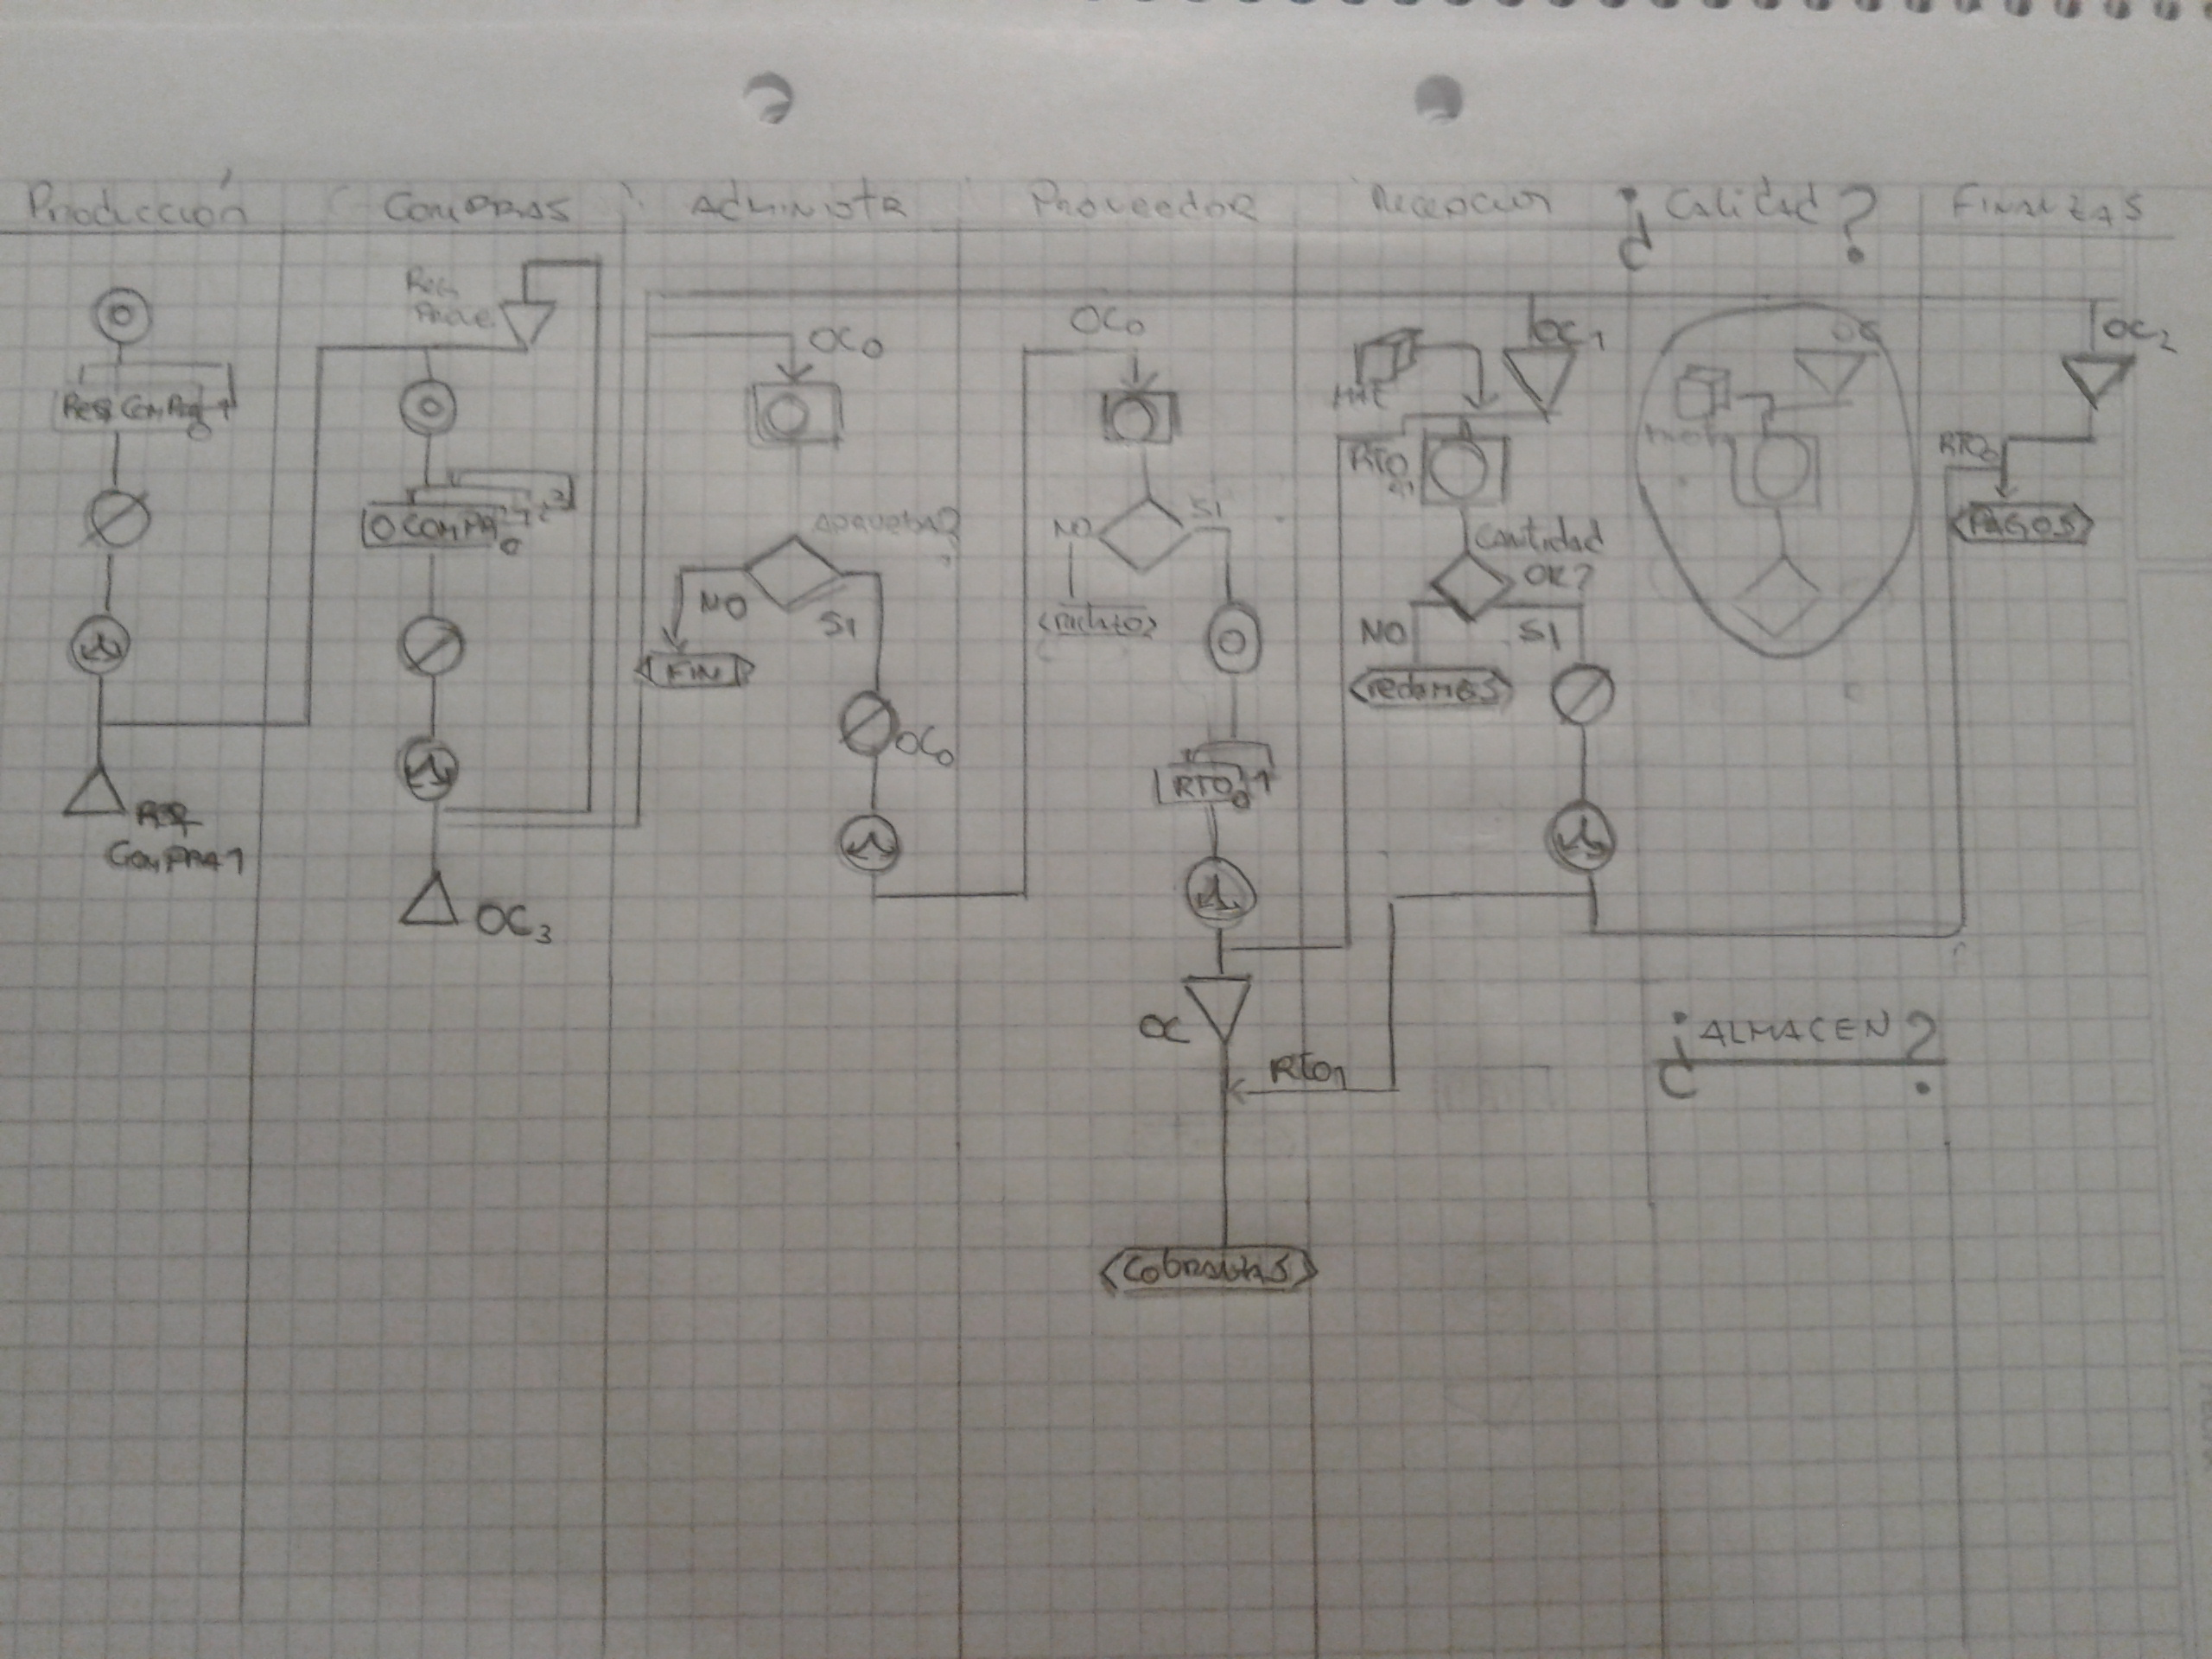
\includegraphics [scale=0.22 ,angle=90]{Empresa/Circuitos/Compras/Compras.jpg}

\pagebreak
\section{Procedimiento de Compras}
\begin{description}
\item[Producción] Tras detectar necesidad de materiales y luego de chequear las existencias, si el stock del sector de Producción alcanza el punto de pedido, este emite un Requerimiento de Compra (RC) en original y copia, el nivel autorizante firma el original y lo envía al sector de Compras, se archiva la copia.
\item[Compras] Recibido el Requerimiento de Compra, el área de Compras consulta catálogos y listas de precios actualizados de los proveedores, y en función de ellos confecciona una Orden de Compra (OC) original y cuatro copias, las firma y distribuye original a Dirección General, una copia a Recepción, una a Finanzas, una a Calidad y almacena la última copia.
\item [Dirección General] Tras recibir la Orden de Compra del sector de Compras, la Dirección General la controla, y en caso de aprobarla la firma y envía al sector de Ventas del Proveedor previamente seleccionado.
\item [Proveedor] Una vez recibida la Orden de Compra firmada por Compras y Dirección General el Proveedor, según su circuito de ventas,  decide aceptar o rechazar la Orden de Compra. En caso de aceptarla, el Proveedor confecciona Remito (Rto) por duplicado y envía original y una copia junto con los materiales al sector de Recepción.
\item[Recepción] Tras recibir los materiales y el Remito original y una copia, el sector de Recepción controla cotejando cantidades en ambos contra la Orden de Compra. En caso de concordar, firma Remito original y copia, distribuye el original al sector Finanzas y devuelve la copia al Proveedor. Envía la mercadería al sector de Calidad para su control.
\item [Proveedor] Recibido el remito firmado continua con su Circuito no relevado de Cobranzas.
\item [Calidad] Recibida la mercadería de Recepción, controla la calidad contra lo especificado en la Orden de Compra. De aprobar, almacena la mercadería. De no aprobar, emite un Reclamo al Proveedor.
\item [Finanzas] Una vez recibido el Remito original del sector de Recepción, procede a realizar el pago en el circuito no relevado de Pago a Proveedores.

\end{description}

\pagebreak
\section{Manual del Cursograma de Compras}


\pagebreak
\section{Formularios de Compras}
\subsection{Formulario1}
imagen
\begin{itemize}
  \item \textbf{Objetivo:}
  \item \textbf{Alcance:}
  \item \textbf{Emisor:}
  \item \textbf{Cantidad de Copias Emitidas:}
  \item \textbf{Sector receptor:}
 \end{itemize}
\subsubsection{Descripci\'on campos del Formulario1}

\subsection{Formulario2}
imagen
\begin{itemize}
  \item \textbf{Objetivo:}
  \item \textbf{Alcance:}
  \item \textbf{Emisor:}
  \item \textbf{Cantidad de Copias Emitidas:}
  \item \textbf{Sector receptor:}
 \end{itemize}
\subsubsection{Descripci\'on campos del Formulario2}

\pagebreak
\section{Normas de Control Interno de Compras}
